\chapter{Design}

\section{Architettura}
L’architettura di MPoly è basata sul pattern architetturale MVC.\newline
Si è scelto di implementare MVC nella sua forma classica in quanto il gioco 
ha una modalità di interazione ad eventi: ovvero ogni modifica che avviene sul model è a seguito di un evento generato
dall'utente.\newline
L’utente interagisce con l' applicazione facendo scaturire un evento (pressione di un bottone nella view, tasto della tastiera\dots).
Il controller cattura questo evento ed esegue una serie di operazioni 
specifiche per la sua gestione interagendo con la parte model dell'app, e susseguentemente aggiorna la view 
mostrando all’utente che cosa è successo.\newline   
In riferimento allo schema dell'architettura, è stato predisposto un controller principale denominato GameManager 
che ha un riferimento a un oggetto che implementa l'interfaccia MainView,
sul quale chiamerà l'aggiornamento della view.\newline
In questa versione dell'applicazione la modalità di interazione utente avviene tramite pressione di bottoni della view.
Per questo si è deciso di implementare il pattern "Observer": MainViewImpl ha un riferimento al GameController ed è questa classe 
che notifica il Controller dell' inizio di un evento.
Al momento della notifica il controller interroga il model.\newline
A seguito dell'analisi sono stati individuati 3 punti d'entrata per la componente model dell'applicazione,
ognuno dei quali si occupa di un macro aspetto del dominio. 
Nello specifico abbiamo:
\begin{itemize}
    \item Board, che si occupa di gestire la struttura del tabellone, le caselle con case e alberghi e il movimento delle 
    pedine.
    \item TurnationManager (che sarebbe il corrispettivo di referee nell'analisi)
    che si occupa di gestire l'avvicendarsi dei turni dei giocatori e la fine del gioco.
    \item Bank, per orchestrare lo scambio di denaro fra i bank account dei giocatori e 
    la compravendita di contratti di proprietà.
\end{itemize} 
Questi punti d’ entrata del model offrono delle primitive che incapsulano la logica di funzionamento 
delle principali azioni che si possono compiere durante il gioco, azioni che sono caratteristiche del 
gioco stesso Monopoly. Il controller orchestra varie chiamate ai metodi di queste 3 classi del model per far funzionare
il gioco.
Con questa architettura il model è perfettamente scorporabile e riutilizzabile per costruire 
un software diverso che risponda allo stesso dominio. L'assenza di un unico punto di entrata per il model
previene l'esistenza di una macro classe con eccesiva responsabilità sulla quale dipenderebbe tutto il funzionamento
del gioco, facilitando lo sviluppo e l'evoluzione del software.\newline
Il controller coopera con model e view mediante delle interfacce che sono completamente indipendenti 
dall’implementazione di quest’ultimi. 
Questo, in particolare, fa sì che le scelte implementative della view non determinino cambiamenti sul 
controller o sul model in alcun caso rendendo dunque totalmente
indipendente e modificabile l'implementazione.
In aggiunta, si potrebbe prevedere l'esistenza di uno specifico componente che implementi il pattern observer con il GameController
e che chiami i metodi di quest'ultimo permettendo altre modalità di interazione (cattura evento pressione dei tasti del mouse, della tastiera\dots)
Il software prevede anche un menù iniziale di configurazione della partita. 
Questo menù è a sua volta costituito da una sua architettura MVC più ridotta, 
seguendo lo stesso pattern Observer. 
L’entità MainController è colei che crea poi le classi del model e l' MVC principale avviando effettivamente il gioco.

\begin{figure}[H]
    \centering
    \makebox[1.0\textwidth]{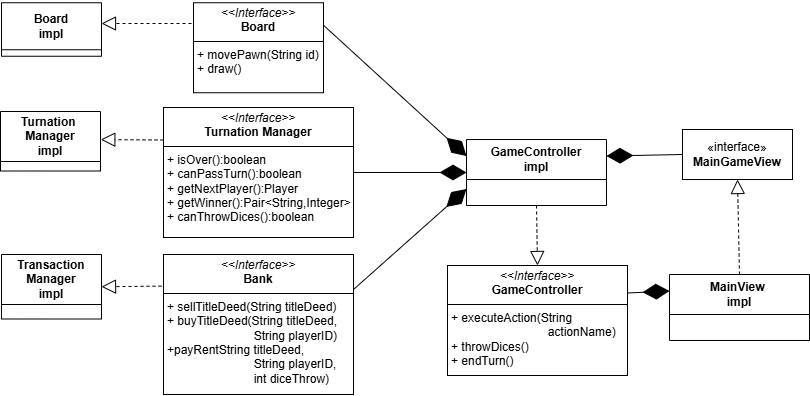
\includegraphics[width=1.3\textwidth]{img/architecture.png}}	
    \caption{Schema UML dell'architettura del software. \texttt{GameControllerImpl} ha un riferimento alla view
    e alle 3 class principali del model. MainViewImpl ha un riferimento al \texttt{GameController}
    implementando il pattern observer}
	\label{img:architecture_diagram}
\end{figure}